\documentclass[11pt,letterpaper]{article}

\usepackage{iftex}
\ifPDFTeX
  \usepackage[T1]{fontenc}
  \usepackage[utf8]{inputenc}
  \usepackage{lmodern}
\else
  \usepackage{fontspec}
  \setmainfont{Latin Modern Roman}
  \setsansfont{Latin Modern Sans}
  \setmonofont{Latin Modern Mono}[Scale=MatchLowercase]
\fi
\usepackage[provide=*,spanish]{babel}
\addto\captionsspanish{\renewcommand{\tablename}{Tabla}}

\usepackage[letterpaper,top=1.75cm,bottom=1.75cm,left=1.85cm,right=1.85cm]{geometry}
\usepackage{graphicx}
% Permite compilar desde informe/ o desde la raíz del repositorio.
\makeatletter
\providecommand*{\input@path}{}
\g@addto@macro\input@path{{informe/}}
\makeatother
\graphicspath{{informe/}}
\usepackage{booktabs}
\usepackage{tabularx}
\usepackage{longtable}
\usepackage{array}
\usepackage{makecell}
\usepackage[table]{xcolor}
\usepackage{enumitem}
\usepackage{listings}
\usepackage{amsmath,amssymb}
\usepackage{microtype}
\usepackage{fancyhdr}
\usepackage{hyperref}
\usepackage{xurl}
\usepackage{caption}
\usepackage{float}

\definecolor{navy}{HTML}{173B63}
\definecolor{paleblue}{HTML}{EAF1F8}
\definecolor{palegray}{HTML}{F4F6F8}
\definecolor{midgray}{HTML}{D9D9D9}
\definecolor{textgray}{HTML}{4B5563}

\hypersetup{
  colorlinks=true,
  linkcolor=navy,
  urlcolor=navy,
  pdftitle={Informe técnico del analizador léxico para un subconjunto de Prolog},
  pdfauthor={Jose Jimenez Saavedra, Franco Oyarzo Calisto y Demian Quezada Pasten}
}

\pagestyle{fancy}
\fancyhf{}
\fancyhead[R]{\sffamily\scriptsize\color{textgray} TEORÍA DE LA COMPUTACIÓN $\mid$ INFORME TÉCNICO}
\fancyfoot[R]{\sffamily\scriptsize\color{textgray} Análisis léxico $\mid$ Página \thepage}
\renewcommand{\headrulewidth}{0pt}
\renewcommand{\footrulewidth}{0pt}
\setlength{\headheight}{14pt}

\setlength{\parindent}{0pt}
\setlength{\parskip}{0.58em}
\renewcommand{\arraystretch}{1.23}
\setcounter{secnumdepth}{2}
\captionsetup{font=small,labelfont=bf,justification=centering}

\newcolumntype{Y}{>{\raggedright\arraybackslash}X}
\newcolumntype{C}[1]{>{\centering\arraybackslash}p{#1}}
\newcolumntype{L}[1]{>{\raggedright\arraybackslash}p{#1}}

\newcommand{\tableheader}[1]{\cellcolor{navy}\color{white}\sffamily\bfseries #1}
\lstdefinestyle{terminal}{
  basicstyle=\ttfamily\footnotesize,
  backgroundcolor=\color{palegray},
  frame=single,
  rulecolor=\color{midgray},
  breaklines=true,
  columns=fullflexible,
  keepspaces=true,
  showstringspaces=false,
  xleftmargin=0.4em,
  xrightmargin=0.4em,
  aboveskip=0.5em,
  belowskip=0.5em
}

% Generado por python scripts/validate.py; no editar manualmente.
\newcommand{\PruebasTotal}{69}
\newcommand{\PruebasValidasBase}{28}
\newcommand{\PruebasInvalidasBase}{12}
\newcommand{\PruebasCLI}{10}
\newcommand{\PruebasRegresion}{19}
\newcommand{\PythonValidacion}{3.14.4}
\newcommand{\FechaValidacion}{2026-09-22}
\newcommand{\TokensValidos}{94}
\newcommand{\ErroresValidos}{0}
\newcommand{\TokensInvalidos}{30}
\newcommand{\ErroresInvalidos}{6}


\begin{document}

\begin{titlepage}
  \thispagestyle{fancy}
  \centering

  \vspace*{1.2cm}
  {\sffamily\bfseries\color{textgray} UNIVERSIDAD CATÓLICA DE TEMUCO\par}

  \vspace{2.6cm}
  {\sffamily\bfseries\LARGE Informe técnico del analizador léxico para un subconjunto de Prolog\par}
  \vspace{0.6cm}
  {\large Teoría de la Computación\par}

  \vspace{2.0cm}
  \begin{tabularx}{0.9\textwidth}{>{\bfseries\sffamily}L{3.7cm}Y}
    \toprule
    \rowcolor{navy}
    \color{white}Dato & \color{white}\bfseries\sffamily Información \\
    \midrule
    Código del curso & INFO1148 \\
    \rowcolor{palegray} Asignatura & Teoría de la Computación \\
    Integrantes & Jose Jimenez Saavedra --- \href{mailto:jose.jimenez2023@alu.uct.cl}{jose.jimenez2023@alu.uct.cl} \\
    & Franco Oyarzo Calisto --- \href{mailto:foyarzo2023@alu.uct.cl}{foyarzo2023@alu.uct.cl} \\
    & Demian Quezada Pasten --- \href{mailto:dquezada2023@alu.uct.cl}{dquezada2023@alu.uct.cl} \\
    \rowcolor{palegray} Profesor & Prof. M. Lévano \\
    Jefe de grupo & Jose Jimenez Saavedra \\
    \rowcolor{palegray} Periodo académico & Segundo semestre de 2026 \\
    \bottomrule
  \end{tabularx}

  \vfill
  {\color{textgray}Temuco, septiembre de 2026\par}
\end{titlepage}
\setcounter{page}{2}

\section*{Resumen}

El trabajo presenta el diseño, la implementación y la validación de un analizador léxico para un subconjunto de Prolog. La solución, desarrollada en Python, recorre la fuente de izquierda a derecha y reconoce átomos, variables, números, cadenas, operadores y delimitadores. Los espacios y comentarios se descartan sin perder el seguimiento de línea y columna. Para resolver lexemas con prefijos compartidos se aplica máxima coincidencia; además, los operadores alfabéticos \texttt{is} y \texttt{mod} se clasifican después de consumir el identificador completo. Cada token conserva su tipo, lexema, posición y, cuando corresponde, un índice en la tabla de lexemas. El signo de los números se trata como operador independiente, de modo que no se confunde el reconocimiento léxico con la interpretación sintáctica. La validación incluye 40 pruebas automatizadas, un programa correcto y otro con errores recuperables. Las pruebas finalizaron sin fallos; el archivo válido produjo 94 tokens y ningún error, mientras que el archivo inválido produjo 30 tokens y seis diagnósticos. El alcance no incluye análisis sintáctico, semántica ni compatibilidad completa con ISO Prolog.

\textit{Palabras clave: análisis léxico, Prolog, autómata finito, máxima coincidencia, tabla de lexemas.}

\section{Introducción}

El análisis léxico transforma una secuencia de caracteres en unidades que pueden ser tratadas por las etapas posteriores de un compilador o intérprete. En este trabajo, el problema consiste en recorrer archivos escritos en un subconjunto de Prolog, distinguir las categorías definidas y asociar a cada token su posición inicial. El recorrido también debe descartar comentarios y espacios sin alterar el cálculo de línea y columna, además de informar errores léxicos sin detenerse ante el primer carácter inválido.

La dificultad no se reduce a comparar caracteres con una lista. Varias categorías comparten prefijos: \verb|\==| comienza como \verb|\=|, \verb|=..| comienza como \verb|=| y el átomo \texttt{island} contiene el prefijo \texttt{is}. Si el analizador aceptara el primer patrón disponible, fragmentaría lexemas que pertenecen a una sola unidad. Por esa razón, la solución conserva la aceptación provisional más larga y aplica una prioridad estable cuando dos reglas pueden reconocer la misma entrada, criterio habitual en la construcción de analizadores léxicos \cite{dragon}.

El informe define primero el subconjunto admitido y sus expresiones regulares. Luego relaciona esas definiciones con AFD para identificadores, números y operadores, e incluye una determinización y una minimización representativas. Las secciones posteriores describen la arquitectura, la tabla de lexemas, el tratamiento de errores y los resultados del corpus automatizado. De este modo, la especificación formal y el comportamiento del programa pueden contrastarse sobre los mismos casos.

\section{Objetivos}

\subsection{Objetivo general}

Desarrollar y validar un analizador léxico para un subconjunto definido de Prolog, relacionando expresiones regulares y autómatas finitos con una implementación en Python capaz de generar tokens posicionados y diagnósticos recuperables.

\subsection{Objetivos específicos}

Los objetivos específicos consisten en definir las categorías admitidas mediante patrones, ejemplos, atributos y reglas de prioridad; modelar categorías representativas con autómatas finitos y documentar una conversión de AFN a AFD junto con su minimización; implementar el recorrido de la fuente, la tabla de lexemas y los diagnósticos de error; y comprobar el comportamiento del analizador mediante pruebas automatizadas y dos archivos completos de entrada.

\section{Alcance del analizador}

La especificación restringe los identificadores y dígitos a caracteres ASCII. Esta decisión mantiene explícitas las clases de transición del autómata y acota la implementación al subconjunto pedido, aunque SWI-Prolog admite identificadores Unicode más amplios \cite{swisyntax}. Los literales citados sí pueden contener otros caracteres, siempre que no introduzcan un salto de línea ni una secuencia de escape fuera de la convención adoptada.

El analizador produce tokens y errores léxicos, pero no determina si esos tokens forman una cláusula correcta. Tampoco interpreta precedencias, realiza unificación, administra ámbitos ni asigna significado a los literales. La Tabla~\ref{tab:alcance} resume esa frontera para evitar que los resultados se presenten como una implementación completa de Prolog.

\begin{table}[H]
\centering
\small
\caption{Decisiones de alcance del analizador.}
\label{tab:alcance}
\begin{tabularx}{\textwidth}{L{2.85cm}YY}
\toprule
\tableheader{Aspecto} & \tableheader{Incluido} & \tableheader{Excluido} \\
\midrule
Identificadores & Átomos iniciados en minúscula; variables iniciadas en mayúscula o guion bajo; \texttt{\_} como anónima. & Unicode fuera de literales citados. \\
\rowcolor{palegray} Números & Enteros, decimales con dígitos a ambos lados del punto y exponentes opcionales. & Bases no decimales, racionales, infinidades y NaN. \\
Texto & Átomos con comillas simples y cadenas dobles; escapes \texttt{\textbackslash n}, \texttt{\textbackslash t}, \texttt{\textbackslash r}, \texttt{\textbackslash\textbackslash}, \texttt{\textbackslash'} y \texttt{\textbackslash"}. & Saltos de línea sin escapar y otros escapes. \\
\rowcolor{palegray} Operadores & Cláusulas, consultas, unificación, comparación, aritmética y control señalados en la tarea. & Operadores definidos por el usuario. \\
Comentarios & \texttt{\%} hasta fin de línea y \texttt{/* ... */}. & Comentarios de bloque anidados. \\
\rowcolor{palegray} Procesamiento & Tokenización, posiciones, tabla de lexemas y recuperación léxica. & Sintaxis, precedencia, unificación, ámbitos y semántica. \\
\bottomrule
\end{tabularx}
\end{table}

\section{Especificación léxica}

Se define $L=[a\text{-}z]$, $U=[A\text{-}Z]$, $D=[0\text{-}9]$ y $C=L\cup U\cup D\cup\{\_\}$. El alfabeto de entrada $\Sigma$ contiene los caracteres Unicode de la fuente, pero los identificadores, dígitos y espacios admitidos se restringen a las clases ASCII indicadas. Los caracteres Unicode adicionales pueden aparecer dentro de citas y comentarios. LF, CRLF y CR se cuentan como un único salto de línea; una tabulación ocupa una columna. Las posiciones comienzan en uno y cuentan caracteres, no bytes ni anchura visual.

Las expresiones de la Tabla~\ref{tab:formal} usan la notación de \texttt{re} de Python: $|$ denota alternativas, los corchetes definen clases y los grupos \texttt{(?:...)} no capturan. Los patrones se aplican desde la posición actual mediante \texttt{match}; no se busca una coincidencia posterior que omita caracteres. En Python las alternativas se intentan de izquierda a derecha, de modo que el orden de operadores largos antes de sus prefijos forma parte de la implementación de máxima coincidencia \cite{pythonre}. Las citas y los comentarios de bloque se recorren explícitamente para conservar el fragmento de los errores de cierre.

\small
\begin{longtable}{L{3.1cm}L{4.7cm}L{7.1cm}}
\caption{Definición formal del subconjunto.}\label{tab:formal}\\
\toprule
\tableheader{Token} & \tableheader{Descripción} & \tableheader{Expresión regular conceptual} \\
\midrule
\endfirsthead
\toprule
\tableheader{Token} & \tableheader{Descripción} & \tableheader{Expresión regular conceptual} \\
\midrule
\endhead
ATOMO & Identificador iniciado en minúscula; se reclasifican \texttt{is} y \texttt{mod}. & \path{[a-z][A-Za-z0-9_]*} \\
\rowcolor{palegray} \makecell[l]{ATOMO\_\\CITADO} & Texto entre comillas simples con escapes admitidos. & \path{'(?:\\[ntr\\'"]|[^'\\\r\n])*'} \\
VARIABLE & Identificador iniciado en mayúscula o guion bajo, excepto el lexema aislado \texttt{\_}. & \path{(?:[A-Z][A-Za-z0-9_]*|_[A-Za-z0-9_]+)} \\
\rowcolor{palegray} \makecell[l]{VARIABLE\_\\ANONIMA} & Guion bajo aislado. & \path{_} \\
ENTERO & Secuencia decimal sin signo. & \path{[0-9]+} \\
\rowcolor{palegray} REAL & Decimal o exponente; el signo solo se admite en el exponente. & \path{(?:[0-9]+\.[0-9]+(?:[eE][+-]?[0-9]+)?|[0-9]+[eE][+-]?[0-9]+)} \\
CADENA & Texto entre comillas dobles con escapes admitidos. & \path{"(?:\\[ntr\\'"]|[^"\\\r\n])*"} \\
\rowcolor{palegray} \makecell[l]{OPERADOR\_\\CLAUSULA} & Operadores de regla y gramática de cláusulas definidas. & \path{-->|:-} \\
\makecell[l]{OPERADOR\_\\CONSULTA} & Inicio de consulta. & \path{\?-} \\
\rowcolor{palegray} \makecell[l]{OPERADOR\_\\COMPARACION} & Unificación, identidad, desigualdad y comparación. & \path{\\==|=\.\.|\\=|==|=<|>=|=|<|>} \\
\makecell[l]{OPERADOR\_\\ARITMETICO} & Operadores simbólicos y alfabéticos admitidos. & \path{//|\*\*|[+\-*/]|is|mod} \\
\rowcolor{palegray} \makecell[l]{OPERADOR\_\\CONTROL} & Negación, corte y disyunción. & \path{\\\+|!|;} \\
DELIMITADORES & Familia de tokens detallada en la Tabla~\ref{tab:delimitadores}. & \path{[()\[\]{}|,.]} \\
\rowcolor{palegray} COMENTARIO de línea & Desde \texttt{\%} hasta antes de CR, LF o fin de archivo; se descarta. & \path{%[^\r\n]*} \\
COMENTARIO de bloque & Hasta el primer cierre; sin anidamiento; se descarta. & \path{/\*[^*]*\*+(?:[^/*][^*]*\*+)*/} \\
\rowcolor{palegray} ESPACIO & Separadores descartados con actualización de posición. & \path{[ \t\r\n\f\v]+} \\
\bottomrule
\end{longtable}
\normalsize

Los operadores cubren los lexemas obligatorios de la tarea y la extensión opcional \texttt{-->}. Prolog permite declarar operadores y asociarles precedencia y tipo, pero esa información pertenece al análisis sintáctico y queda fuera de este lexer \cite{swioperators}. Se reconoce primero el identificador completo: solo los lexemas exactos \texttt{is} y \texttt{mod} se reclasifican como operadores; \texttt{island}, \texttt{modulo} e \texttt{is2} son átomos. Entre números válidos, REAL tiene prioridad sobre ENTERO. El signo inicial siempre es un operador: \texttt{-25} produce dos tokens, mientras que \texttt{2e-3} produce un REAL.

Ambas clases de citas permiten contenido vacío y los escapes \verb|\n|, \verb|\t|, \verb|\r|, \verb|\\|, \verb|\'| y \verb|\"|. Se conserva el lexema exacto, incluidas comillas y barras, sin evaluar los escapes. Un CR o LF literal interrumpe una cita sin cierre. Los comentarios no se reconocen dentro de citas; las comillas no tienen significado especial dentro de comentarios. La expresión de bloque impide consumir un cierre intermedio, por lo que \texttt{/* a */ b /* c */} contiene dos comentarios separados por el átomo \texttt{b}.

La aceptación numérica incorpora una regla de frontera: una letra ASCII, guion bajo o un segundo punto seguido de dígito ASCII inmediatamente después del número origina un diagnóstico de número mal formado. Así, \texttt{12abc} y \texttt{3.14.15} no se fragmentan en tokens válidos. Un punto sin dígito posterior queda disponible como PUNTO: \texttt{12.} produce ENTERO y PUNTO. Esta comprobación y la recuperación de errores complementan los patrones de números válidos; no analizan la gramática de cláusulas.

\begin{table}[H]
\centering
\small
\caption{Nombres concretos de los tokens delimitadores. Cada patrón es un carácter literal.}
\label{tab:delimitadores}
\begin{tabularx}{\textwidth}{Y C{1.3cm} Y C{1.3cm}}
\toprule
\tableheader{Token} & \tableheader{Lexema} & \tableheader{Token} & \tableheader{Lexema} \\
\midrule
PARENTESIS\_IZQ & \texttt{(} & PARENTESIS\_DER & \texttt{)} \\
\rowcolor{palegray} CORCHETE\_IZQ & \texttt{[} & CORCHETE\_DER & \texttt{]} \\
LLAVE\_IZQ & \texttt{\{} & LLAVE\_DER & \texttt{\}} \\
\rowcolor{palegray} BARRA\_VERTICAL & \texttt{|} & COMA & \texttt{,} \\
PUNTO & \texttt{.} & & \\
\bottomrule
\end{tabularx}
\end{table}

Los ejemplos inválidos de la Tabla~\ref{tab:ejemplos} no pertenecen a la categoría de su fila; algunos sí son válidos como otra categoría. Por ejemplo, \texttt{Padre} es una variable y \texttt{\_\_} también. Los comentarios y espacios no emiten tokens ni atributos; los índices de átomos, variables y literales comienzan en cero dentro de sus respectivas tablas.

\small
\begin{longtable}{L{3.1cm}L{3.3cm}L{4.3cm}L{3.5cm}}
\caption{Ejemplos y atributos asociados.}\label{tab:ejemplos}\\
\toprule
\tableheader{Token} & \tableheader{Ejemplos válidos} & \tableheader{Ejemplos inválidos} & \tableheader{Atributo} \\
\midrule
\endfirsthead
\toprule
\tableheader{Token} & \tableheader{Ejemplos válidos} & \tableheader{Ejemplos inválidos} & \tableheader{Atributo} \\
\midrule
\endhead
ATOMO & \texttt{padre}, \texttt{persona\_1} & \texttt{Padre}, \texttt{1persona} & Índice en átomos \\
\rowcolor{palegray} \makecell[l]{ATOMO\_\\CITADO} & \texttt{'Juan Pérez'}, \texttt{':-'} & \texttt{'sin cierre} & Índice en átomos \\
VARIABLE & \texttt{X}, \texttt{Persona}, \texttt{\_Tmp} & \texttt{x}, \texttt{2X} & Índice en variables \\
\rowcolor{palegray} \makecell[l]{VARIABLE\_\\ANONIMA} & \texttt{\_} & \texttt{\_\_} como anónima & Sin índice \\
ENTERO & \texttt{25}, \texttt{0} & \texttt{12abc}, \texttt{2e} & Índice en literales \\
\rowcolor{palegray} REAL & \texttt{3.14}, \texttt{2e-3} & \texttt{3.14.15}, \texttt{1e+} & Índice en literales \\
CADENA & \texttt{"hola"}, \verb|"a\n b"| & \texttt{"sin cierre}, \verb|"x\q"| & Índice en literales \\
\rowcolor{palegray} \makecell[l]{OPERADOR\_\\CLAUSULA} & \texttt{:-}, \texttt{-->} & \texttt{:}, \texttt{?-} & Sin índice \\
\makecell[l]{OPERADOR\_\\CONSULTA} & \texttt{?-} & \texttt{?}, \texttt{:-} & Sin índice \\
\rowcolor{palegray} \makecell[l]{OPERADOR\_\\COMPARACION} & \verb|\==|, \texttt{=..}, \texttt{=<} & \texttt{is}, \texttt{@} & Sin índice \\
\makecell[l]{OPERADOR\_\\ARITMETICO} & \texttt{//}, \texttt{**}, \texttt{is} & \texttt{island}, \texttt{=} & Sin índice \\
\rowcolor{palegray} \makecell[l]{OPERADOR\_\\CONTROL} & \verb|\+|, \texttt{!}, \texttt{;} & \texttt{+}, \texttt{?} & Sin índice \\
DELIMITADORES & \texttt{( ) [ ] \{ \} | , .} & \texttt{@}, \texttt{\#} & Sin índice \\
\rowcolor{palegray} COMENTARIO & \texttt{\% nota}, \texttt{/* nota */} & \texttt{/* sin cierre} & Se descarta \\
ESPACIO & Espacio, TAB, CR, LF, FF, VT & Espacio Unicode U+00A0 & Se descarta \\
\bottomrule
\end{longtable}
\normalsize

\section{Diseño de los autómatas}

Los autómatas de las Figuras~\ref{fig:identificadores}, \ref{fig:numeros} y \ref{fig:operadores} representan las categorías con mayor posibilidad de superposición. La flecha de entrada identifica el estado inicial $q_0$ y la doble circunferencia identifica los estados aceptadores, con la categoría indicada en su interior. Las transiciones omitidas llevan a un estado muerto implícito. Al tokenizar, se conserva la última aceptación y se devuelve el prefijo aceptado más largo; el carácter que inicia el siguiente token queda sin consumir. La validación de fronteras numéricas puede sustituir ese prefijo por un diagnóstico, según la especificación anterior.

\begin{figure}[H]
  \centering
  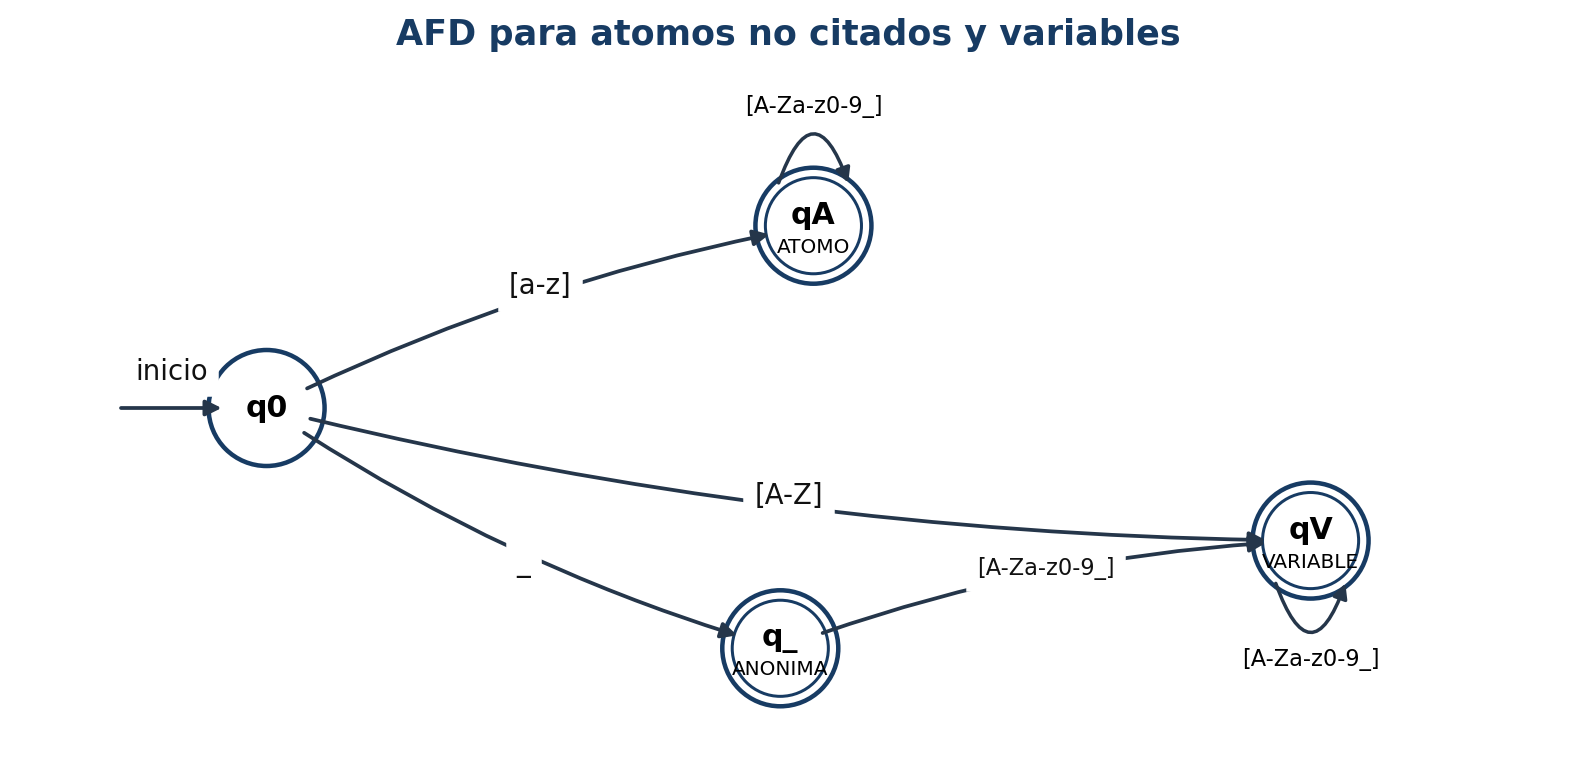
\includegraphics[width=0.98\textwidth]{figuras/afd_identificadores.png}
  \caption{AFD para identificadores. El estado $q_A$ requiere reclasificar \texttt{is} y \texttt{mod}.}
  \label{fig:identificadores}
\end{figure}

\begin{figure}[H]
  \centering
  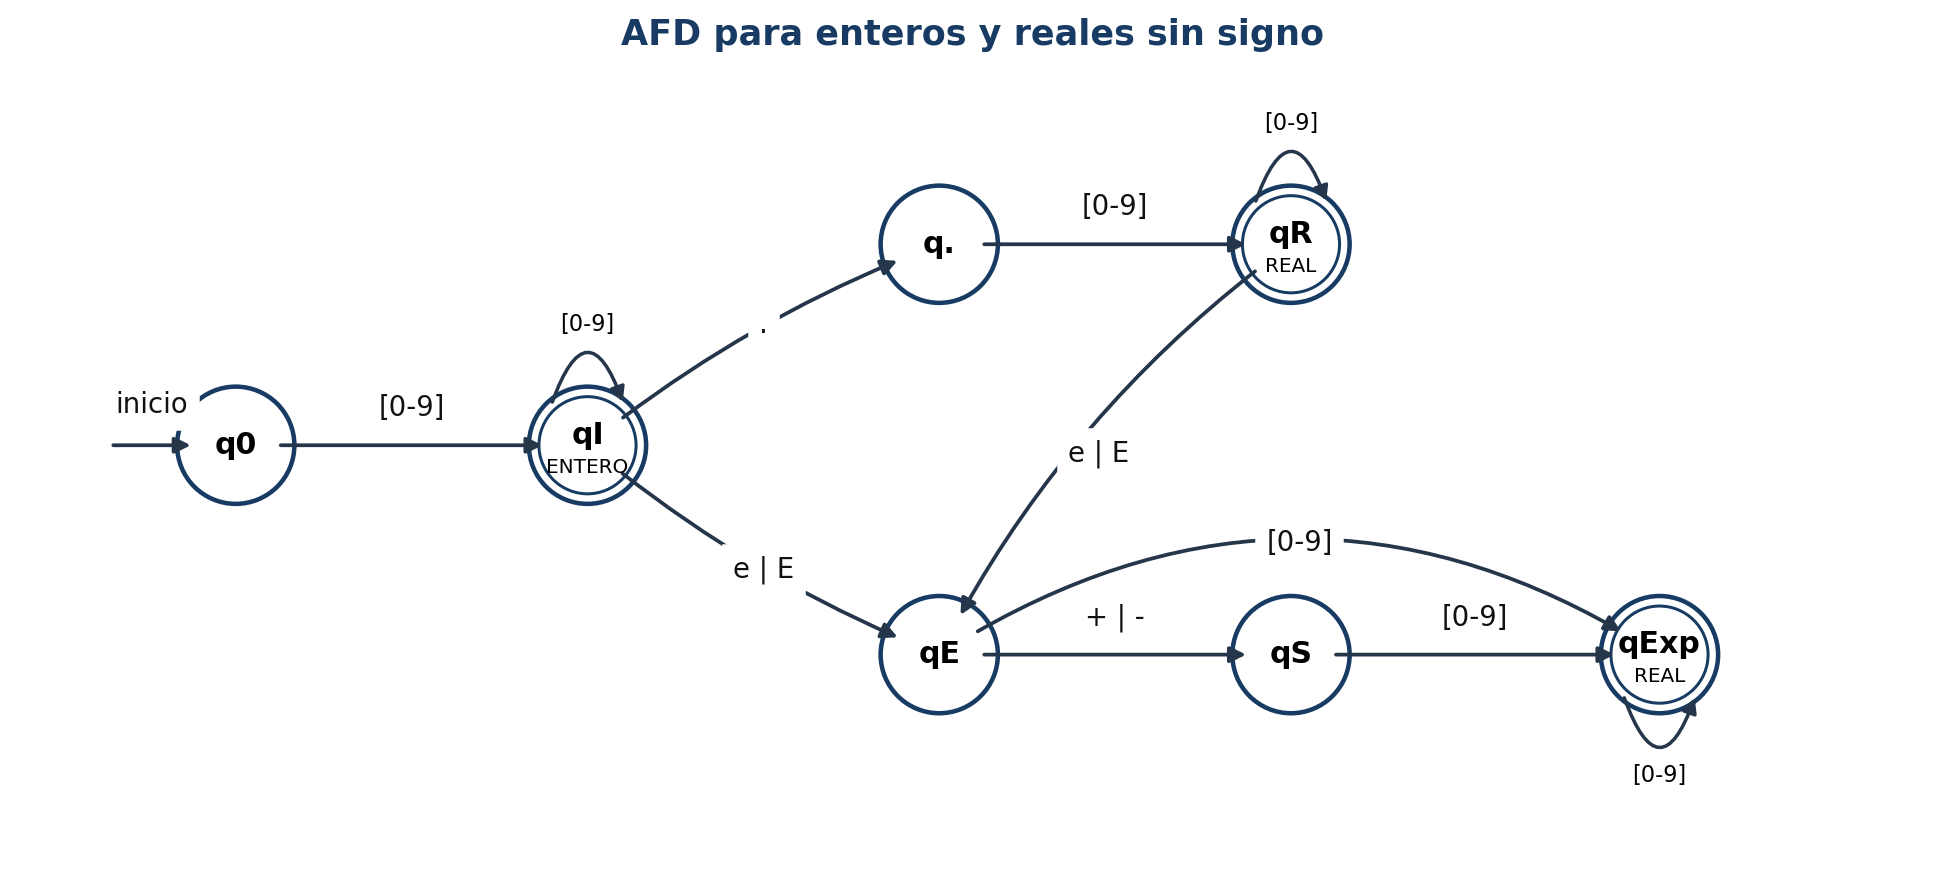
\includegraphics[width=0.98\textwidth]{figuras/afd_numeros.png}
  \caption{AFD para enteros y reales sin signo léxico.}
  \label{fig:numeros}
\end{figure}

\begin{figure}[H]
  \centering
  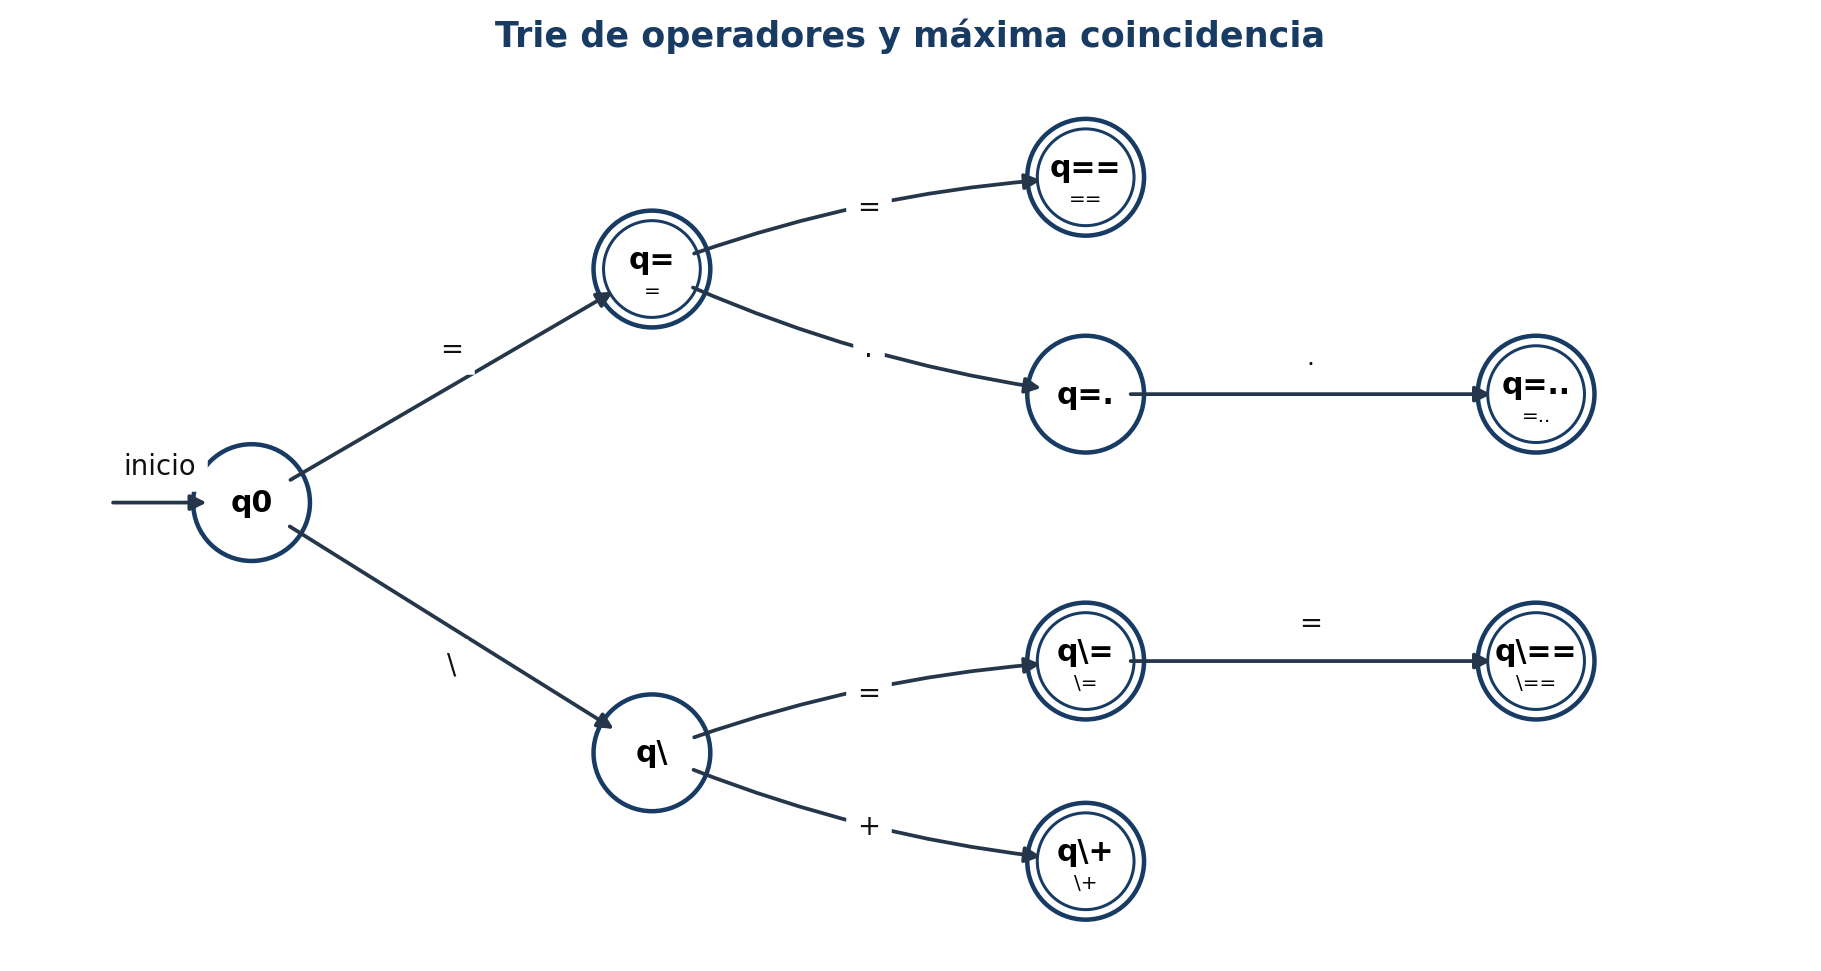
\includegraphics[width=0.98\textwidth]{figuras/afd_operadores.png}
  \caption{Fragmento del trie de operadores con prefijos compartidos.}
  \label{fig:operadores}
\end{figure}

El estado $q_{\_}$ acepta únicamente la variable anónima. Si se lee otro carácter de $C$, se pasa a $q_V$ y el lexema completo es una variable con nombre. En el autómata numérico, $q_I$, $q_R$ y $q_{Exp}$ aceptan ENTERO, REAL y REAL, respectivamente; $q_{.}$, $q_E$ y $q_S$ no aceptan. Por ejemplo, \texttt{2e-3} recorre $q_0,q_I,q_E,q_S,q_{Exp}$. Para \texttt{12.}, la última aceptación es $q_I$: el punto queda como delimitador. Para \texttt{1e+}, la frontera detecta un exponente incompleto y produce un error, en lugar de emitir el entero \texttt{1}.

El trie mostrado es un fragmento: \texttt{=} y \verb|\=| ya aceptan, pero pueden prolongarse hasta \texttt{==}, \texttt{=..} y \verb|\==|. En el lexer, la tupla completa \texttt{SYMBOL\_OPERATORS}, ordenada por longitud descendente, representa las demás ramas. Un delimitador requiere una transición desde el inicio a su estado aceptador; espacios y comentarios terminados alcanzan estados de descarte.

\subsection{Autómatas para citas y comentarios}

Un mismo AFD sirve para ATOMO\_CITADO y CADENA parametrizando la comilla $c$ (simple o doble). Sea $E=\{n,t,r,\backslash,\text{comilla simple},\text{comilla doble}\}$ el conjunto permitido después de una barra. La Tabla~\ref{tab:afd-citas} especifica todas las transiciones que no van al estado muerto. $Q_0$ es inicial y $Q_F$ es el único aceptador: emite el tipo determinado por $c$. Las clases de cada fila son disjuntas; en $Q_I$ la comilla opuesta es un carácter ordinario.

\begin{table}[H]
\centering
\small
\caption{AFD parametrizado para átomos citados y cadenas.}
\label{tab:afd-citas}
\begin{tabularx}{\textwidth}{C{1.5cm}Y C{1.5cm} L{4.0cm}}
\toprule
\tableheader{Origen} & \tableheader{Entrada} & \tableheader{Destino} & \tableheader{Interpretación} \\
\midrule
$Q_0$ & $c$ & $Q_I$ & Apertura \\
\rowcolor{palegray} $Q_I$ & $\Sigma\setminus\{c,\backslash,\mathrm{CR},\mathrm{LF}\}$ & $Q_I$ & Contenido ordinario \\
$Q_I$ & $\backslash$ & $Q_E$ & Inicio de escape \\
\rowcolor{palegray} $Q_E$ & $E$ & $Q_I$ & Escape admitido \\
$Q_I$ & $c$ & $Q_F$ & Cierre y aceptación \\
\bottomrule
\end{tabularx}
\end{table}

CR, LF o fin de archivo antes de $Q_F$ generan un diagnóstico de cita sin cierre. Un escape fuera de $E$ impide aceptar el literal; la implementación conserva la primera secuencia inválida y continúa hasta su cierre o fin de línea para recuperar el análisis. Este recorrido de recuperación no convierte el literal erróneo en un token aceptado.

Para comentarios de línea, el estado inicial $L_0$ pasa con \texttt{\%} a $L_1$, que es aceptador y repite con $\Sigma\setminus\{\mathrm{CR},\mathrm{LF}\}$. Al encontrar un salto o fin de archivo se descarta el comentario. El salto queda para el reconocedor de espacios. Para comentarios de bloque, la Tabla~\ref{tab:afd-bloque} reconoce el primer cierre \texttt{*/}; $B_0$ es inicial y $B_F$ es el único aceptador. Un fin de archivo en $B_2$ o $B_3$ produce un error de comentario sin cierre. La entrada \texttt{/*} activa este reconocedor antes que el operador \texttt{/}.

\begin{table}[H]
\centering
\small
\caption{Transiciones no muertas del AFD de comentarios de bloque.}
\label{tab:afd-bloque}
\begin{tabularx}{\textwidth}{C{1.5cm}Y C{1.5cm} L{4.0cm}}
\toprule
\tableheader{Origen} & \tableheader{Entrada} & \tableheader{Destino} & \tableheader{Interpretación} \\
\midrule
$B_0$ & \texttt{/} & $B_1$ & Primer carácter \\
\rowcolor{palegray} $B_1$ & \texttt{*} & $B_2$ & Apertura completa \\
$B_2$ & $\Sigma\setminus\{\texttt{*}\}$ & $B_2$ & Contenido \\
\rowcolor{palegray} $B_2$ & \texttt{*} & $B_3$ & Posible cierre \\
$B_3$ & \texttt{*} & $B_3$ & Mantiene posible cierre \\
\rowcolor{palegray} $B_3$ & $\Sigma\setminus\{\texttt{*},\texttt{/}\}$ & $B_2$ & Continúa contenido \\
$B_3$ & \texttt{/} & $B_F$ & Cierre y descarte \\
\bottomrule
\end{tabularx}
\end{table}

\subsection{Determinización representativa}

Para mostrar la construcción de subconjuntos se utiliza el lenguaje $LC^*$ de identificadores iniciados en minúscula, antes de reclasificar las palabras \texttt{is} y \texttt{mod}. En este ejemplo, la etiqueta ATOMO designa ese patrón estructural. Se parte de un AFN deliberadamente no mínimo que divide la primera letra en dos ramas equivalentes. El estado $q_0$ posee transiciones $\varepsilon$ hacia $p_0$ y $r_0$; desde $p_0$, una letra de $[a\text{-}m]$ lleva a $p_1$, mientras que desde $r_0$ una letra de $[n\text{-}z]$ lleva a $r_1$. Los estados $p_1$ y $r_1$ son aceptadores y repiten con cualquier carácter de $C$. La transformación aplica la construcción de subconjuntos y luego refina particiones para obtener estados equivalentes \cite{hopcroft}.

Formalmente, $Q=\{q_0,p_0,r_0,p_1,r_1\}$, el inicial es $q_0$ y $F=\{p_1,r_1\}$. Las clases de entrada son $[a\text{-}m]$, $[n\text{-}z]$, $U\cup D\cup\{\_\}$ y $\Sigma\setminus C$. Para esta última, todas las transiciones del AFN son vacías; se omite su columna para facilitar la lectura.

\begin{table}[H]
\centering
\small
\caption{Transiciones del AFN representativo.}
\label{tab:afn}
\begin{tabularx}{0.92\textwidth}{C{1.7cm}C{2.1cm}C{2.1cm}C{2.1cm}Y}
\toprule
\tableheader{Estado} & \tableheader{$\varepsilon$} & \tableheader{$[a$--$m]$} & \tableheader{$[n$--$z]$} & \tableheader{$U\cup D\cup\{\_\}$} \\
\midrule
$q_0$ & $\{p_0,r_0\}$ & $\varnothing$ & $\varnothing$ & $\varnothing$ \\
\rowcolor{palegray} $p_0$ & $\varnothing$ & $\{p_1\}$ & $\varnothing$ & $\varnothing$ \\
$r_0$ & $\varnothing$ & $\varnothing$ & $\{r_1\}$ & $\varnothing$ \\
\rowcolor{palegray} $p_1$ & $\varnothing$ & $\{p_1\}$ & $\{p_1\}$ & $\{p_1\}$ \\
$r_1$ & $\varnothing$ & $\{r_1\}$ & $\{r_1\}$ & $\{r_1\}$ \\
\bottomrule
\end{tabularx}
\end{table}

Para un subconjunto $S$ y un carácter $a$ se calcula
\[
\delta_D(S,a)=\operatorname{cl}_{\varepsilon}
\left(\bigcup_{q\in S}\delta_N(q,a)\right).
\]
La clausura-$\varepsilon$ inicial es $D_0=\{q_0,p_0,r_0\}$. Al mover ese conjunto con $[a\text{-}m]$ se obtiene $D_1=\{p_1\}$; con $[n\text{-}z]$ se obtiene $D_2=\{r_1\}$. Cualquier clase sin transición conduce a $D_{\bot}=\varnothing$. Como $p_1$ y $r_1$ repiten con $C$, no aparecen nuevos subconjuntos. Un subconjunto acepta si intersecta $F$, por lo que solo $D_1$ y $D_2$ son aceptadores. Los cuatro estados son alcanzables: con $\varepsilon$, \texttt{a}, \texttt{n} y \texttt{0}, respectivamente.

\begin{table}[H]
\centering
\small
\caption{Tabla de transición obtenida mediante construcción de subconjuntos.}
\label{tab:determinizado}
\begin{tabularx}{\textwidth}{L{3.4cm}C{1.9cm}C{1.9cm}C{3.3cm}Y}
\toprule
\tableheader{Estado AFD} & \tableheader{$[a$--$m]$} & \tableheader{$[n$--$z]$} & \tableheader{$U\cup D\cup\{\_\}$} & \tableheader{Aceptación} \\
\midrule
$D_0=\{q_0,p_0,r_0\}$ & $D_1$ & $D_2$ & $D_{\bot}$ & No \\
\rowcolor{palegray} $D_1=\{p_1\}$ & $D_1$ & $D_1$ & $D_1$ & ATOMO \\
$D_2=\{r_1\}$ & $D_2$ & $D_2$ & $D_2$ & ATOMO \\
\rowcolor{palegray} $D_{\bot}=\varnothing$ & $D_{\bot}$ & $D_{\bot}$ & $D_{\bot}$ & No \\
\bottomrule
\end{tabularx}
\end{table}

Para todo estado de la Tabla~\ref{tab:determinizado}, una entrada de $\Sigma\setminus C$ conduce a $D_{\bot}$. Por ejemplo, \texttt{padre\_1} sigue $D_0,D_2,D_2,D_2,D_2,D_2,D_2,D_2$ y acepta; \texttt{Padre} pasa inmediatamente al estado muerto. No se confunde rechazo como átomo con error global: el despachador reconoce \texttt{Padre} mediante el AFD de variables.

\subsection{Minimización}

La partición inicial es $P_0=\{\{D_1,D_2\},\{D_0,D_{\bot}\}\}$: el primer bloque contiene los estados que aceptan ATOMO y el segundo, los que no aceptan. El bloque no aceptador se divide porque desde $D_0$ una letra minúscula alcanza aceptación, mientras que desde $D_{\bot}$ toda entrada permanece en el estado muerto. En cambio, $D_1$ y $D_2$ no se separan: ambos aceptan exactamente los sufijos de $C^*$ y cualquier carácter fuera de $C$ lleva al mismo estado muerto. La partición estable es $P_1=\{\{D_1,D_2\},\{D_0\},\{D_{\bot}\}\}$, por lo que $D_1$ y $D_2$ se fusionan en la clase de equivalencia $D_A=[D_1]=[D_2]$.

Los tres estados restantes son distinguibles: el sufijo vacío $\varepsilon$ separa $D_A$ de ambos estados no aceptadores, y el sufijo \texttt{a} distingue $D_0$ de $D_{\bot}$. Como todos son alcanzables, el AFD completo de tres estados es mínimo. En los diagramas parciales se omite el estado muerto y quedan dos estados visibles para este patrón. Esta minimización no corresponde al lexer entero: un AFD que emita varias categorías debe conservar las etiquetas de token al formar su partición inicial.

\begin{table}[H]
\centering
\small
\caption{AFD mínimo para el ejemplo representativo.}
\label{tab:minimo}
\begin{tabularx}{\textwidth}{L{3.4cm}C{1.9cm}C{1.9cm}C{3.3cm}Y}
\toprule
\tableheader{Estado mínimo} & \tableheader{$[a$--$m]$} & \tableheader{$[n$--$z]$} & \tableheader{$U\cup D\cup\{\_\}$} & \tableheader{Aceptación} \\
\midrule
$D_0$ & $D_A$ & $D_A$ & $D_{\bot}$ & No \\
\rowcolor{palegray} $D_A=[D_1]=[D_2]$ & $D_A$ & $D_A$ & $D_A$ & ATOMO \\
$D_{\bot}$ & $D_{\bot}$ & $D_{\bot}$ & $D_{\bot}$ & No \\
\bottomrule
\end{tabularx}
\end{table}

Las entradas de $\Sigma\setminus C$ llevan a $D_{\bot}$ también en la Tabla~\ref{tab:minimo}. La reclasificación de \texttt{is} y \texttt{mod} se mantiene después del reconocimiento: fusionar los estados estructurales no elimina la consulta del lexema completo.

\subsection{Estrategia integrada y correspondencia con el código}

\subsubsection{Trazas de aceptación y fronteras}

Las siguientes trazas separan la aceptación del autómata de la decisión del lexer sobre la frontera del lexema. Un estado no aceptador intermedio no implica que toda la entrada sea errónea: puede existir una aceptación anterior. A su vez, la regla numérica de frontera puede impedir emitir ese prefijo si ocultaría un número mal formado.

\begin{table}[H]
\centering
\small
\caption{Trazas representativas y resultado observable.}
\begin{tabularx}{\textwidth}{L{2cm}Y L{5.5cm}}
\toprule
\tableheader{Entrada} & \tableheader{Recorrido relevante} & \tableheader{Resultado del lexer} \\
\midrule
\texttt{12.} & $q_0,q_I,q_I,q_{.}$. La última aceptación está antes del punto. & ENTERO \texttt{12}, PUNTO \texttt{.}. \\
\rowcolor{palegray} \texttt{2e-3} & $q_0,q_I,q_E,q_S,q_{Exp}$. El signo pertenece al exponente. & Un REAL con lexema \texttt{2e-3}. \\
\texttt{1e+} & $q_0,q_I,q_E,q_S$. El estado final no acepta y el sufijo inicia con \texttt{e}. & Un error por \texttt{1e+}; no se emite ENTERO. \\
\rowcolor{palegray} \texttt{3.14.15} & Se alcanza $q_R$ en \texttt{3.14}; la frontera siguiente es punto más dígito. & Un error por todo \texttt{3.14.15}. \\
\texttt{\_X} & $q_0,q_{\_},q_V$. La aceptación de variable prolonga la anónima. & VARIABLE con índice; no se emite \texttt{\_} separado. \\
\rowcolor{palegray} \texttt{is2} & $q_0,q_A,q_A,q_A$. Se consulta el lexema completo. & ATOMO, porque no coincide exactamente con \texttt{is}. \\
\bottomrule
\end{tabularx}
\end{table}

Los casos numéricos se verifican en \path{tests/test_lexer.py} y \path{tests/test_lexer_regressions.py}. Estos archivos también contrastan operadores adyacentes sin espacios, prefijos incompletos y la prioridad de las citas sobre los marcadores de comentario. El caso \texttt{)][(,;.} se acepta léxicamente aunque no forme una cláusula: comprobar el orden de los delimitadores sería análisis sintáctico y queda fuera del enunciado.

\subsubsection{Despacho de reconocedores}

El programa no materializa un AFD único en memoria. Utiliza una estrategia equivalente: un despachador selecciona la categoría a partir del carácter inicial. Primero descarta espacios y comentarios; después reconoce citas, números e identificadores; finalmente intenta operadores, delimitadores y el diagnóstico de carácter no admitido. Las expresiones \texttt{IDENTIFIER}, \texttt{REAL} e \texttt{INTEGER} describen los lenguajes de sus AFD, y \texttt{SYMBOL\_OPERATORS} codifica las hojas del trie. Esto establece equivalencia de reconocimiento; no afirma que el motor \texttt{re} de Python ejecute internamente un AFD.

Las superposiciones se resuelven de manera explícita: \texttt{/*} tiene prioridad sobre \texttt{/}; una cita consume su interior antes de reconocer operadores; un identificador se completa antes de reclasificar palabras; y los operadores se prueban por longitud descendente. Todos los reconocedores aceptan un lexema, descartan un separador o producen un diagnóstico que avanza la lectura. El ciclo principal conserva una sola posición y termina cuando llega al final de la fuente. Así se relacionan los autómatas, las reglas de prioridad y la recuperación sin incorporar análisis sintáctico.

\section{Reglas de prioridad y máxima coincidencia}

\begin{table}[H]
\centering
\small
\caption{Resolución de superposiciones entre patrones.}
\label{tab:prioridad}
\begin{tabularx}{\textwidth}{L{2.7cm}YL{4.3cm}}
\toprule
\tableheader{Caso} & \tableheader{Regla aplicada} & \tableheader{Resultado} \\
\midrule
\texttt{\textbackslash== / \textbackslash= / ==} & Los operadores se prueban por longitud descendente. El lexer no confirma \texttt{\textbackslash=} si existe otro signo igual consecutivo. & \texttt{\textbackslash==} cuando la entrada es \texttt{\textbackslash==}. \\
\rowcolor{palegray} \texttt{=.. / =} & Tras reconocer \texttt{=} como aceptación provisional, se continúa por dos puntos si están disponibles. & \texttt{=..} cuando la entrada es \texttt{=..}. \\
\texttt{:- / :} & Solo \texttt{:-} pertenece al subconjunto. Un \texttt{:} aislado genera un diagnóstico. & \texttt{:-} o error en \texttt{:}. \\
\rowcolor{palegray} \texttt{\_ / \_Variable} & Se reconoce primero el identificador completo. Solo el lexema exacto \texttt{\_} se clasifica como anónimo. & VARIABLE\_ANONIMA o VARIABLE. \\
\texttt{is / island} & Se consume la palabra completa y después se consulta la tabla de operadores alfabéticos. & \makecell[l]{OPERADOR\_\\ARITMETICO o ATOMO.} \\
\rowcolor{palegray} \texttt{-25} & El signo queda fuera del patrón numérico y se emite como operador independiente. & \texttt{-} seguido de ENTERO \texttt{25}. \\
\bottomrule
\end{tabularx}
\end{table}

La implementación aplica estas reglas dentro de un orden de decisión único. Primero reconoce espacios y comentarios, porque no deben producir tokens. Después procesa los literales citados, los números y los identificadores. Los operadores simbólicos se comparan por longitud descendente y los delimitadores se dejan para el final. Si ninguna categoría acepta el carácter actual, se registra un error y se avanza una posición.

Esta secuencia evita dos problemas concretos. Un comentario de bloque debe detectarse antes del operador división, y una palabra completa debe reconocerse antes de decidir si corresponde a \texttt{is}, \texttt{mod} o a un átomo ordinario. La prioridad, por tanto, no reemplaza la máxima coincidencia; ambas reglas trabajan juntas.

\section{Diseño e implementación}

\subsection{Arquitectura de la solución}

\begin{table}[H]
\centering
\small
\caption{Componentes de la implementación.}
\label{tab:arquitectura}
\begin{tabularx}{\textwidth}{L{3cm}L{3.6cm}Y}
\toprule
\tableheader{Archivo} & \tableheader{Componente} & \tableheader{Responsabilidad} \\
\midrule
\path{src/lexer.py} & \texttt{Token} y \texttt{LexError} & Representan salidas inmutables con tipo, lexema, posición y atributo opcional. \\
\rowcolor{palegray} \path{src/lexer.py} & \texttt{SymbolTable} & Interna átomos, variables y literales; reutiliza el índice de un lexema repetido. \\
\path{src/lexer.py} & \texttt{Lexer.scan} & Recorre la fuente una vez, aplica prioridad, actualiza posiciones y recupera errores. \\
\rowcolor{palegray} \path{src/cli.py} & Interfaz CLI & Lee UTF-8 con BOM opcional y emite texto o JSON en UTF-8; retorna 0, 1 o 2 según el resultado. \\
\path{tests/} & Pruebas & Comprueba categorías, posiciones, recuperación, interfaz y corpus completo. \\
\rowcolor{palegray} \path{corpus/} & Entradas completas & Contiene un programa sin errores y otro con varios errores recuperables. \\
\path{scripts/validate.py} & Evidencia reproducible & Ejecuta la suite y el corpus; actualiza resultados JSON y cifras del informe. \\
\bottomrule
\end{tabularx}
\end{table}

La interfaz carga el archivo como texto UTF-8, acepta un BOM inicial opcional y lo entrega a \texttt{Lexer.scan} sin alterar sus saltos de línea. El recorrido mantiene el índice absoluto, la línea y la columna. Antes de consumir un lexema guarda su posición inicial; después actualiza el contador con el texto realmente leído. Los identificadores y números se reconocen mediante patrones compilados, mientras que los literales citados y comentarios de bloque se procesan manualmente para distinguir cierre, salto de línea y escape. Los operadores simbólicos se consultan en una secuencia ordenada desde el lexema más largo. Los códigos de salida son 0 si no hay errores léxicos, 1 si se detectaron errores recuperables o hasta EOF, y 2 ante un archivo ilegible, UTF-8 inválido o argumentos incorrectos.

El resultado agrupa la lista de tokens, la lista de errores y la tabla de lexemas. La interfaz puede imprimir tokens en el formato solicitado o serializar el resultado completo en JSON. Como cada carácter consumido hace avanzar el índice y la cantidad de operadores es fija, el costo del recorrido crece linealmente con el tamaño de la entrada. Los errores consumen el fragmento problemático y el análisis continúa cuando existe un límite de recuperación identificable.

\subsection{Formato de salida}

El siguiente fragmento proviene de \path{corpus/programa_valido.pl}. El quinto campo corresponde al índice de la tabla de lexemas cuando la categoría lo utiliza.

\begin{lstlisting}[style=terminal]
<ATOMO, 'padre', 2, 1, 0>
<PARENTESIS_IZQ, '(', 2, 6>
<ATOMO, 'juan', 2, 7, 1>
<COMA, ',', 2, 11>
<ATOMO, 'ana', 2, 13, 2>
<PARENTESIS_DER, ')', 2, 16>
<PUNTO, '.', 2, 17>
\end{lstlisting}

\subsection{Tabla de lexemas}

La tabla usa diccionarios que conservan un índice por primera aparición. Los átomos no citados y citados comparten una tabla; las variables poseen otra; y los enteros, reales y cadenas se registran como pares \texttt{(tipo, lexema)}, lo que evita mezclar valores escritos de forma distinta. Se conserva la escritura original: \texttt{juan} y \texttt{'juan'} tienen entradas distintas, y no se interpretan los escapes ni se convierten números a valores de Python. Los índices son locales a cada tabla y comienzan en cero; el tipo del token identifica cuál debe consultarse. La variable anónima no se interna porque cada aparición representa una variable nueva y no debe compartir identidad.

\begin{table}[H]
\centering
\small
\caption{Ejemplo de internación sin duplicados.}
\label{tab:lexemas}
\begin{tabularx}{\textwidth}{L{2.5cm}YL{4.5cm}}
\toprule
\tableheader{Tabla} & \tableheader{Ejemplo} & \tableheader{Regla} \\
\midrule
Átomos & \texttt{padre $\rightarrow$ 0; juan $\rightarrow$ 1; ana $\rightarrow$ 2} & El mismo lexema reutiliza el índice. \\
\rowcolor{palegray} Variables & \texttt{X $\rightarrow$ 0; Z $\rightarrow$ 1; Y $\rightarrow$ 2} & \texttt{\_} se excluye. \\
Literales & \texttt{(ENTERO, 52) $\rightarrow$ 0} y \texttt{(CADENA, "Ana Perez") $\rightarrow$ 1} & El tipo y la escritura forman la clave. \\
\bottomrule
\end{tabularx}
\end{table}

\section{Tratamiento de errores léxicos}

\begin{longtable}{L{3.2cm}L{2.3cm}L{4.7cm}L{4.5cm}}
\caption{Errores, mensajes y estrategia de recuperación.}\label{tab:errores}\\
\toprule
\tableheader{Error} & \tableheader{Ejemplo} & \tableheader{Mensaje} & \tableheader{Recuperación} \\
\midrule
\endfirsthead
\toprule
\tableheader{Error} & \tableheader{Ejemplo} & \tableheader{Mensaje} & \tableheader{Recuperación} \\
\midrule
\endhead
Átomo citado sin cierre & \texttt{'juan} & \texttt{1:1 Atomo citado sin cierre} & Consume hasta salto de línea o EOF y continúa. \\
\rowcolor{palegray} Cadena sin cierre & \texttt{"hola} & \texttt{1:1 Cadena sin cierre} & Consume hasta salto de línea o EOF y continúa. \\
Comentario sin cierre & \verb|/* texto| & \texttt{1:1 Comentario de bloque sin cierre} & Consume hasta EOF; no existe un límite seguro posterior. \\
\rowcolor{palegray} Carácter no admitido & \texttt{@} & \texttt{1:1 Caracter no admitido} & Consume un carácter y continúa. \\
Número con sufijo & \texttt{12abc} & \texttt{1:1 Numero mal formado} & Consume el fragmento ASCII; conserva el punto que no preceda a un dígito. \\
\rowcolor{palegray} Exponente incompleto & \texttt{2e} & \texttt{1:1 Numero mal formado} & Consume el fragmento numérico completo. \\
Puntos repetidos & \texttt{3.14.15} & \texttt{1:1 Numero mal formado} & Consume el fragmento numérico completo. \\
\rowcolor{palegray} Escape no admitido & \verb|"x\q"| & \texttt{1:1 Secuencia de escape no admitida} & Consume hasta la comilla de cierre. \\
\bottomrule
\end{longtable}

\section{Plan de pruebas y resultados}

Los resultados se generaron el \FechaValidacion{} con Python \PythonValidacion{} mediante \path{scripts/validate.py}. La ejecución automatizada, reproducida en el anexo, completó \PruebasTotal{} pruebas con estado \texttt{OK}. Se conservan \PruebasValidasBase{} pruebas válidas y \PruebasInvalidasBase{} pruebas de entradas inválidas, posiciones o recuperación del corpus original; se añaden \PruebasRegresion{} pruebas de regresión del lexer y \PruebasCLI{} pruebas de la interfaz. El archivo válido produjo \TokensValidos{} tokens y \ErroresValidos{} errores; el archivo con errores produjo \TokensInvalidos{} tokens, \ErroresInvalidos{} diagnósticos y código de salida 1. Las cifras se incorporan desde \path{resultados.tex}, generado a partir de la ejecución, y el registro detallado queda en \path{docs/validation.json}.

\footnotesize
\begin{longtable}{C{0.9cm}L{2.6cm}L{2.75cm}L{3.0cm}L{3.0cm}C{1.3cm}}
\caption{Selección representativa del corpus automatizado.}\label{tab:pruebas}\\
\toprule
\tableheader{ID} & \tableheader{Entrada} & \tableheader{Objetivo} & \tableheader{Esperado} & \tableheader{Obtenido} & \tableheader{Estado} \\
\midrule
\endfirsthead
\toprule
\tableheader{ID} & \tableheader{Entrada} & \tableheader{Objetivo} & \tableheader{Esperado} & \tableheader{Obtenido} & \tableheader{Estado} \\
\midrule
\endhead
P01 & \texttt{padre} & Átomo simple & ATOMO & ATOMO & OK \\
\rowcolor{palegray} P03 & \texttt{'Juan Perez'} & Átomo citado & \makecell[l]{ATOMO\_\\CITADO} & \makecell[l]{ATOMO\_\\CITADO} & OK \\
P07 & \texttt{\_} & Anónima sin índice & \makecell[l]{VARIABLE\_\\ANONIMA} & \makecell[l]{VARIABLE\_\\ANONIMA} & OK \\
\rowcolor{palegray} P10 & \texttt{2e-3} & Real con exponente & REAL & REAL & OK \\
P16 & \verb|\==| & Máxima coincidencia & \verb|\==| & \verb|\==| & OK \\
\rowcolor{palegray} P24 & \texttt{is island} & Límite de palabra & OP / ATOMO & OP / ATOMO & OK \\
P27 & \texttt{padre(X)} repetido & Sin duplicados & Índices 0 y 0 & Índices 0 y 0 & OK \\
\rowcolor{palegray} P29 & \texttt{'juan} & Cierre faltante & Error & Error recuperado & OK \\
P31 & \verb|/* texto| & Comentario abierto & Error & Error hasta EOF & OK \\
\rowcolor{palegray} P33 & \texttt{12abc} & Número mal formado & Error & Error recuperado & OK \\
P35 & \texttt{3.14.15} & Dos puntos & Error & Error recuperado & OK \\
\rowcolor{palegray} P38 & \verb|a.\n  @| & Ubicación & 2:3 & 2:3 & OK \\
P39 & \texttt{1e+} & Exponente incompleto & Fragmento \texttt{1e+} & Fragmento \texttt{1e+} & OK \\
\rowcolor{palegray} P40 & \texttt{12abc, ok.} & Recuperación numérica & \texttt{, ok .} & \texttt{, ok .} & OK \\
\bottomrule
\end{longtable}
\normalsize

\subsection{Análisis de resultados}

El registro JSON incluye huellas SHA-256 de los archivos de código, pruebas, corpus y del propio validador. Antes de calcularlas se normalizan los finales CRLF a LF para comparar copias entre plataformas. El validador comprueba que estas entradas no hayan cambiado durante la ejecución. Las huellas permiten identificar el contenido probado y detectar evidencia desactualizada; no acreditan autoría ni sustituyen las contribuciones registradas en Git.

La cobertura comprueba cada familia léxica, los límites entre palabras y operadores, la deduplicación de lexemas y la actualización de líneas y columnas. Los casos P16 y P24 muestran que la prioridad no se resuelve solo por el orden de las alternativas: primero se consume el lexema completo y después se clasifica. Los casos P39 y P40 verifican que un exponente incompleto se reporte como un solo fragmento y que el analizador retome el reconocimiento en el delimitador siguiente.

El archivo con errores confirma una recuperación parcial. Después de \texttt{@}, \texttt{12abc}, una cadena abierta al final de línea, \texttt{3.14.15} y un escape inválido, el lexer vuelve a reconocer tokens posteriores. En cambio, un comentario de bloque abierto consume hasta el final del archivo porque no existe una marca léxica segura que indique dónde habría terminado.

Las regresiones verifican además saltos LF, CRLF y CR, preservación del punto de cláusula después de números mal formados y fragmentos de literales que terminan en una barra invertida. La interfaz se comprueba ejecutando procesos reales: formato solicitado en el enunciado, referencias a la tabla de lexemas, recuperación en el corpus inválido, BOM UTF-8, texto Unicode incluso con salida redirigida, archivo vacío, ayuda, archivo inexistente y codificación inválida. Un error de lectura genera un diagnóstico de uso y código 2 sin una traza interna de Python.

La principal limitación está en el alcance: el programa usa identificadores ASCII y no intenta reproducir toda la sintaxis de SWI-Prolog. Tampoco decide si una secuencia de tokens forma una cláusula válida. En consecuencia, los resultados demuestran conformidad con el subconjunto definido en este informe, no compatibilidad total con ISO Prolog.

\section{Conclusiones}

El analizador cumple el objetivo planteado para el subconjunto definido: reconoce las categorías obligatorias, conserva la posición inicial de cada token, registra átomos, variables y literales sin duplicados innecesarios, y comunica los errores junto con el fragmento que los produce. Esta conclusión se apoya en \PruebasTotal{} pruebas automatizadas finalizadas sin fallos y en dos ejecuciones completas. El programa válido produjo \TokensValidos{} tokens sin diagnósticos; el programa inválido permitió recuperar \TokensInvalidos{} tokens y reportó \ErroresInvalidos{} errores.

La máxima coincidencia resultó decisiva en los operadores con prefijos compartidos. Sin ella, \verb|\==| podría dividirse como \verb|\=| y \texttt{=}, mientras que \texttt{=..} podría reducirse prematuramente a \texttt{=}. La clasificación posterior de identificadores resolvió un problema distinto: \texttt{is} se reconoce como operador aritmético, pero \texttt{island} permanece como átomo. También se optó por tratar el signo como operador independiente, decisión que mantiene la etapa léxica separada de la interpretación sintáctica de una expresión.

El alcance sigue siendo limitado de forma deliberada. Se admiten identificadores ASCII, un conjunto acotado de escapes y números decimales, pero no todas las extensiones de SWI-Prolog. Un comentario de bloque abierto consume hasta el final del archivo porque no existe un cierre seguro desde el cual reanudar el recorrido. Como trabajo posterior, la solución podría incorporar identificadores Unicode, otras formas numéricas y la generación automática de tablas de transición a partir de una especificación única. Esas ampliaciones tendrían que acompañarse de nuevas pruebas y de la actualización del modelo formal para conservar la coherencia alcanzada.

\begin{thebibliography}{9}

\bibitem{dragon}
Aho, A. V., Lam, M. S., Sethi, R., y Ullman, J. D. (2007). \textit{Compilers: Principles, techniques, and tools} (2.ª ed.). Pearson.

\bibitem{hopcroft}
Hopcroft, J. E., Motwani, R., y Ullman, J. D. (2007). \textit{Introduction to automata theory, languages, and computation} (3.ª ed.). Pearson.

\bibitem{pythonre}
Python Software Foundation. (2026). \textit{re --- Regular expression operations}. Documentación de Python 3. Recuperado el 22 de septiembre de 2026 de \url{https://docs.python.org/3/library/re.html}

\bibitem{swisyntax}
SWI-Prolog. (s. f.). \textit{The SWI-Prolog syntax}. Recuperado el 22 de septiembre de 2026 de \url{https://www.swi-prolog.org/pldoc/man?section=syntax}

\bibitem{swioperators}
SWI-Prolog. (s. f.). \textit{Operators}. Recuperado el 22 de septiembre de 2026 de \url{https://www.swi-prolog.org/pldoc/man?section=operators}

\end{thebibliography}

\section{Anexos}

\begin{table}[H]
\centering
\small
\caption{Recursos asociados al informe.}
\label{tab:recursos}
\begin{tabularx}{\textwidth}{L{4cm}Y}
\toprule
\tableheader{Recurso} & \tableheader{Ubicación o enlace} \\
\midrule
Repositorio Git & \textit{Enlace que debe incorporarse desde el repositorio definitivo del grupo.} \\
\rowcolor{palegray} Código principal & \path{src/lexer.py} y \path{src/cli.py}. \\
Pruebas & \path{tests/test_lexer.py}. \\
\rowcolor{palegray} Corpus & \path{corpus/programa_valido.pl} y \path{corpus/programa_con_errores.pl}. \\
\bottomrule
\end{tabularx}
\end{table}

\subsection{Evidencia de ejecución}

\begin{lstlisting}[style=terminal]
$ python -m unittest discover -s tests -v
Ran 40 tests in 0.001s
OK

$ python -m src.cli corpus/programa_valido.pl --json
94 tokens | 0 errores | codigo de salida 0

$ python -m src.cli corpus/programa_con_errores.pl --json
30 tokens | 6 errores | codigo de salida 1
\end{lstlisting}

\subsection{Registro de contribuciones}

El registro definitivo debe extraerse del historial del repositorio, ya que la trazabilidad exige asociar actividades con commits existentes. Los campos se mantienen abiertos porque el material revisado no incluye un repositorio Git ni evidencia que permita atribuir tareas individuales. Cada integrante debe conocer la solución completa, aunque el desarrollo se distribuya.

\begin{table}[H]
\centering
\small
\caption{Registro que debe completarse con el historial Git del grupo.}
\label{tab:contribuciones}
\begin{tabularx}{\textwidth}{L{4.3cm}YY}
\toprule
\tableheader{Integrante} & \tableheader{Actividad realizada} & \tableheader{Commit o evidencia} \\
\midrule
Jose Jimenez Saavedra & \rule{4.0cm}{0.3pt} & \rule{4.0cm}{0.3pt} \\
\rowcolor{palegray} Franco Oyarzo Calisto & \rule{4.0cm}{0.3pt} & \rule{4.0cm}{0.3pt} \\
Demian Quezada Pasten & \rule{4.0cm}{0.3pt} & \rule{4.0cm}{0.3pt} \\
\bottomrule
\end{tabularx}
\end{table}


\end{document}
